\documentclass{beamer}
\usetheme{Madrid}
\usepackage[utf8]{inputenc}
\usepackage[portuguese]{babel}
\usepackage[T1]{fontenc}
\usepackage{amsmath}
\usepackage{amsfonts}
\usepackage{amssymb}
\usepackage{tikz}
\usepackage{pdfpages}
\usepackage{graphicx}
\author{Dingchao Gao}
\title{Quantum Circuit Transformation For Neutral atom computation}
% \subtitle{QCT for NA}
\setbeamercovered{transparent} 
%\setbeamertemplate{navigation symbols}{} 
%\logo{\includegraphics[scale=.7]{LogoCentralDataShow}} 
\institute{ISCAS} 
\date{\today} 
%\subject{} 
\usepackage{xcolor}
\definecolor{darkorange}{rgb}{1.0, 0.55, 0.0} 

\tikzset{
    DasAtomStyle/.style={color=black, ultra thick},
    TetrisStyle/.style={color=darkorange,ultra thick, dashed},
    EnolaStyle/.style={color=green!50!black,ultra thick, dotted},
    AtomiqueStyle/.style={color=red!70!black, ultra thick, loosely dash dot}
}
\usetikzlibrary{calc,patterns}
\usetikzlibrary{shapes.geometric, arrows, positioning}
\usepackage{pgfplots}

\AtBeginSection[]
{
\begin{frame}{contents}
\transfade
\tableofcontents[sectionstyle=show/shaded,subsectionstyle=show/shaded/hide]
\addtocounter{framenumber}{-1} 
\end{frame}
}

\begin{document}
% \Large

% Title page

\begin{frame}
    \titlepage
\end{frame}
\begin{frame}{Main reference}
    \begin{itemize}
        \item \href{https://arxiv.org/abs/2309.08656}{Computational Capabilities and Compiler Development for Neutral Atom Quantum Processors: Connecting Tool Developers and Hardware Experts}
        \item \href{https://arxiv.org/abs/2409.03185}{DasAtom: A Divide-and-Shuttle Atom Approach to Quantum Circuit Transformation,Yunqi Huang and Dingchao Gao and Shenggang Ying and Sanjiang Li}
    \end{itemize}
\end{frame}
\section{Background}

\subsection{Hardware Characteristics of Atom-Based Quantum Computing}
\begin{frame}
\frametitle{Recent Developments}

\begin{itemize}
    % \item \textbf{Atom Computing's 1,000+ Qubit Quantum Computer} \\
    % \href{https://www.atom-computing.com/news/atom-computing-unveils-1000-qubit-quantum-computer}{\footnotesize{atom-computing.com/news/atom-computing-unveils-1000-qubit-quantum-computer}}
    
    \item \textbf{Microsoft and Atom Computing Collaboration} \\
    \href{https://www.microsoft.com/en-us/research/blog/microsoft-and-atom-computing-collaborate-on-quantum-supercomputer}{\footnotesize{microsoft.com/en-us/research/blog/microsoft-and-atom-computing-collaborate-on-quantum-supercomputer}}
    
    \item \textbf{Modular Quantum System-on-Chip Development} \\
    \href{https://www.nature.com/articles/s41586-024-07371-7}{\footnotesize{nature.com/articles/s41586-024-03876-9}}
    
    \item \textbf{Fault-Tolerant Quantum Computation with High-Rate qLDPC Codes} \\
    \href{https://arxiv.org/abs/2408.12345}{\footnotesize{arxiv.org/abs/2408.12345}}
\end{itemize}
\end{frame}

% \begin{frame}{Neutral Atoms as Qubits}
%   \begin{itemize}
%     \item \textbf{Why Neutral Atoms?}
%       \begin{itemize}
%         \item \textbf{Long Coherence Times:}
%           \begin{itemize}
%             \item Weak interaction with the environment reduces decoherence.
%             \item Enables longer quantum operations.
%           \end{itemize}
%         \item \textbf{High Scalability Potential:}
%           \begin{itemize}
%             \item Optical lattices and tweezers can trap large arrays of atoms.
%             \item Facilitates the creation of highly parallel quantum systems.
%           \end{itemize}
%         \item \textbf{Precise State Control:}
%           \begin{itemize}
%             \item Advanced laser techniques allow for accurate manipulation.
%             \item High-fidelity quantum gate operations.
%           \end{itemize}
%         \item \textbf{Low Cross-Talk:}
%           \begin{itemize}
%             \item Individual addressing minimizes interference between qubits.
%             \item Enhances the reliability of quantum computations.
%           \end{itemize}
%         \item \textbf{Established Technology:}
%           \begin{itemize}
%             \item Builds upon decades of atomic physics research.
%             \item Well-understood cooling and trapping methods.
%           \end{itemize}
%       \end{itemize}
%     \item \textbf{Qubit Representation:}
%       \begin{itemize}
%         \item Specific electronic states (e.g., hyperfine states).
%         \item Use of Rydberg states for entanglement and two-qubit gates.
%       \end{itemize}
%   \end{itemize}
%   % Uncomment to include an illustrative figure
%   % \includegraphics[width=0.8\textwidth]{neutral_atoms_as_qubits.pdf}
% \end{frame}

% Slide: Introduction
\begin{frame}{Neutral Atom Quantum Computing Devices}
    \begin{itemize}
        \item \textbf{Qubits:} Individual neutral atoms (e.g., rubidium, cesium)
        \item \textbf{Trapping Methods:} Optical tweezers, optical lattices
        \item \textbf{Encoding:} Internal atomic states (hyperfine ground states)
        \item \textbf{Interactions:} Mediated via Rydberg state excitation
    \end{itemize}
\end{frame}

% Slide: Key Features
\begin{frame}{Key Features}
    \begin{itemize}
        \item \textbf{Scalability:} Potential for large qubit arrays
        \item \textbf{Long Coherence Times:} Use of clock states reduces sensitivity to magnetic fields
        \item \textbf{Controlled Interactions:} Tunable via Rydberg excitations
    \end{itemize}
\end{frame}

\begin{frame}{Common Atoms Used}
  \begin{itemize}
    \item \textbf{Alkali Atoms} Rubidium (Rb), Cesium (Cs)
    \item \textbf{Alkaline-Earth-Like Atoms} Strontium (Sr),Ytterbium (Yb)
  \end{itemize}
  \centering
  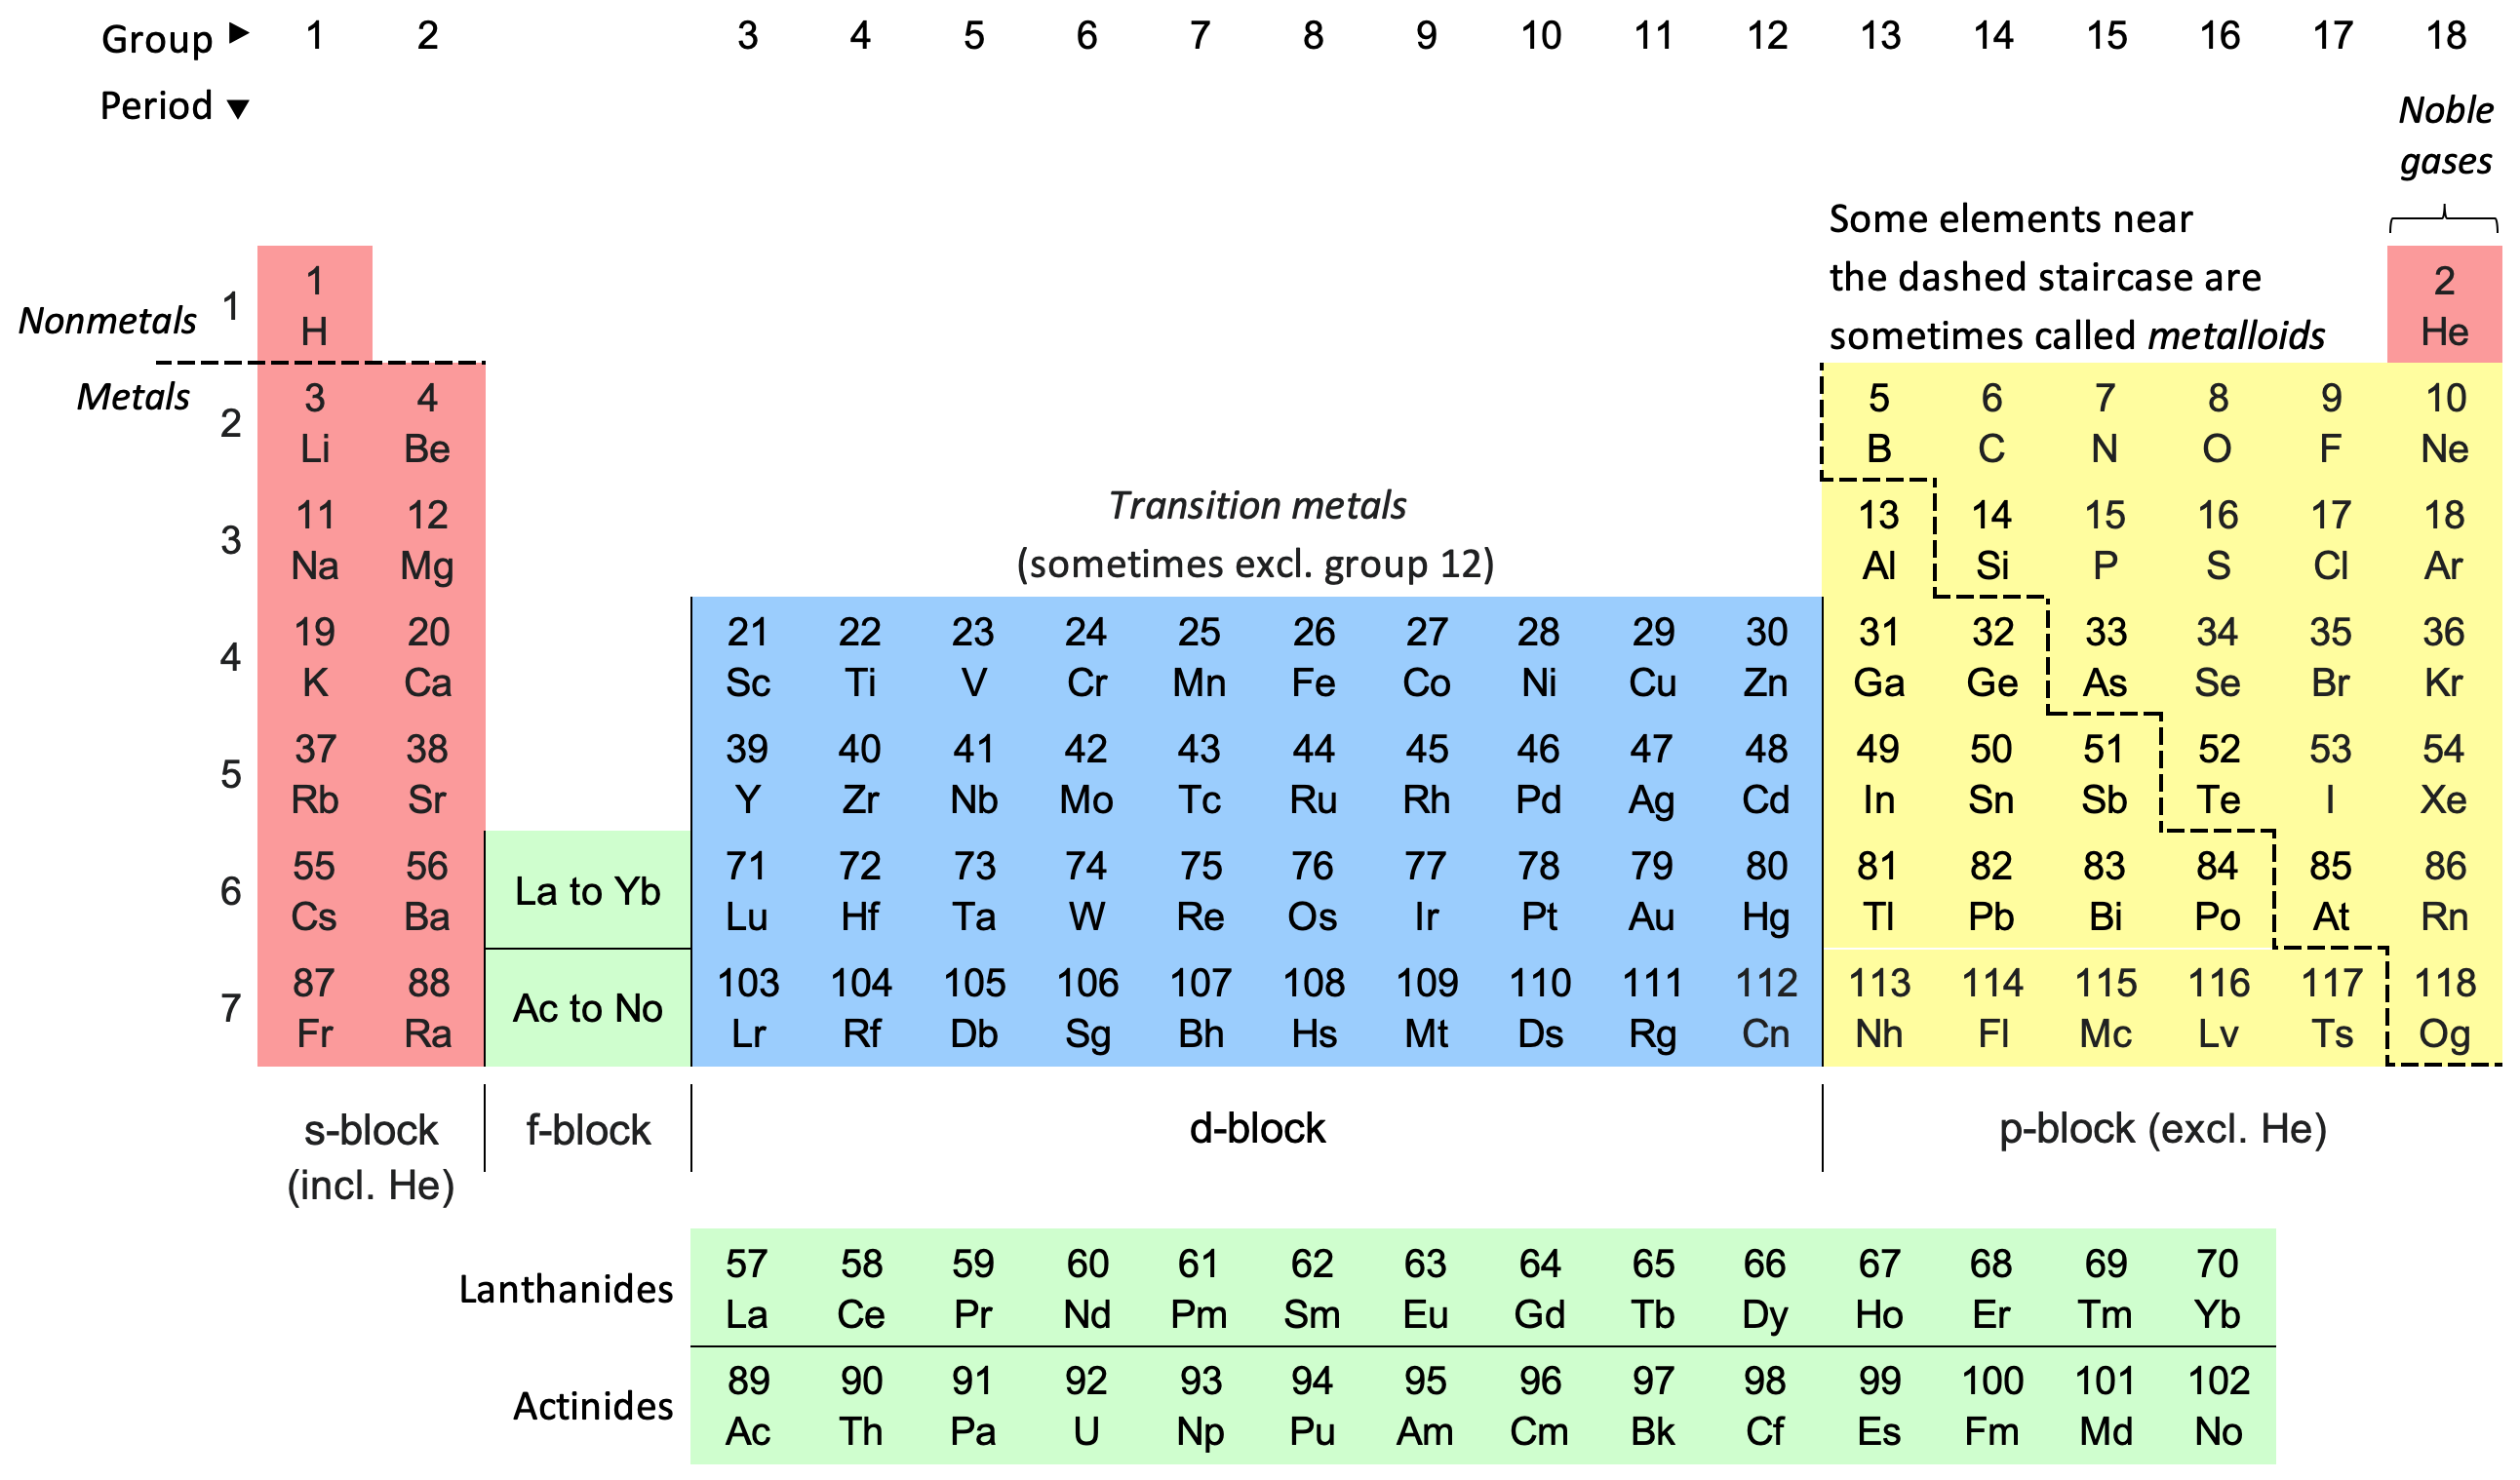
\includegraphics[width=0.7\textwidth]{images/Colour_18-col_PT_with_labels.png}
\end{frame}
\begin{frame}{Workflow}
    \begin{columns}
        \begin{column}{.3\textwidth}
            \begin{enumerate}
                \item Metal
                \item Atomic beam
                \item Cooling
                    % \begin{itemize}
                    %     \item Zeeman slower
                    %     % \item 2D MOT
                    %     % \item 3D MOT
                    %     \item MOT cooling
                    % \end{itemize}
                \item Optical lattice
                \item Rearrange
            \end{enumerate}
        \end{column}
        \begin{column}{.7\textwidth}
            \begin{figure}
                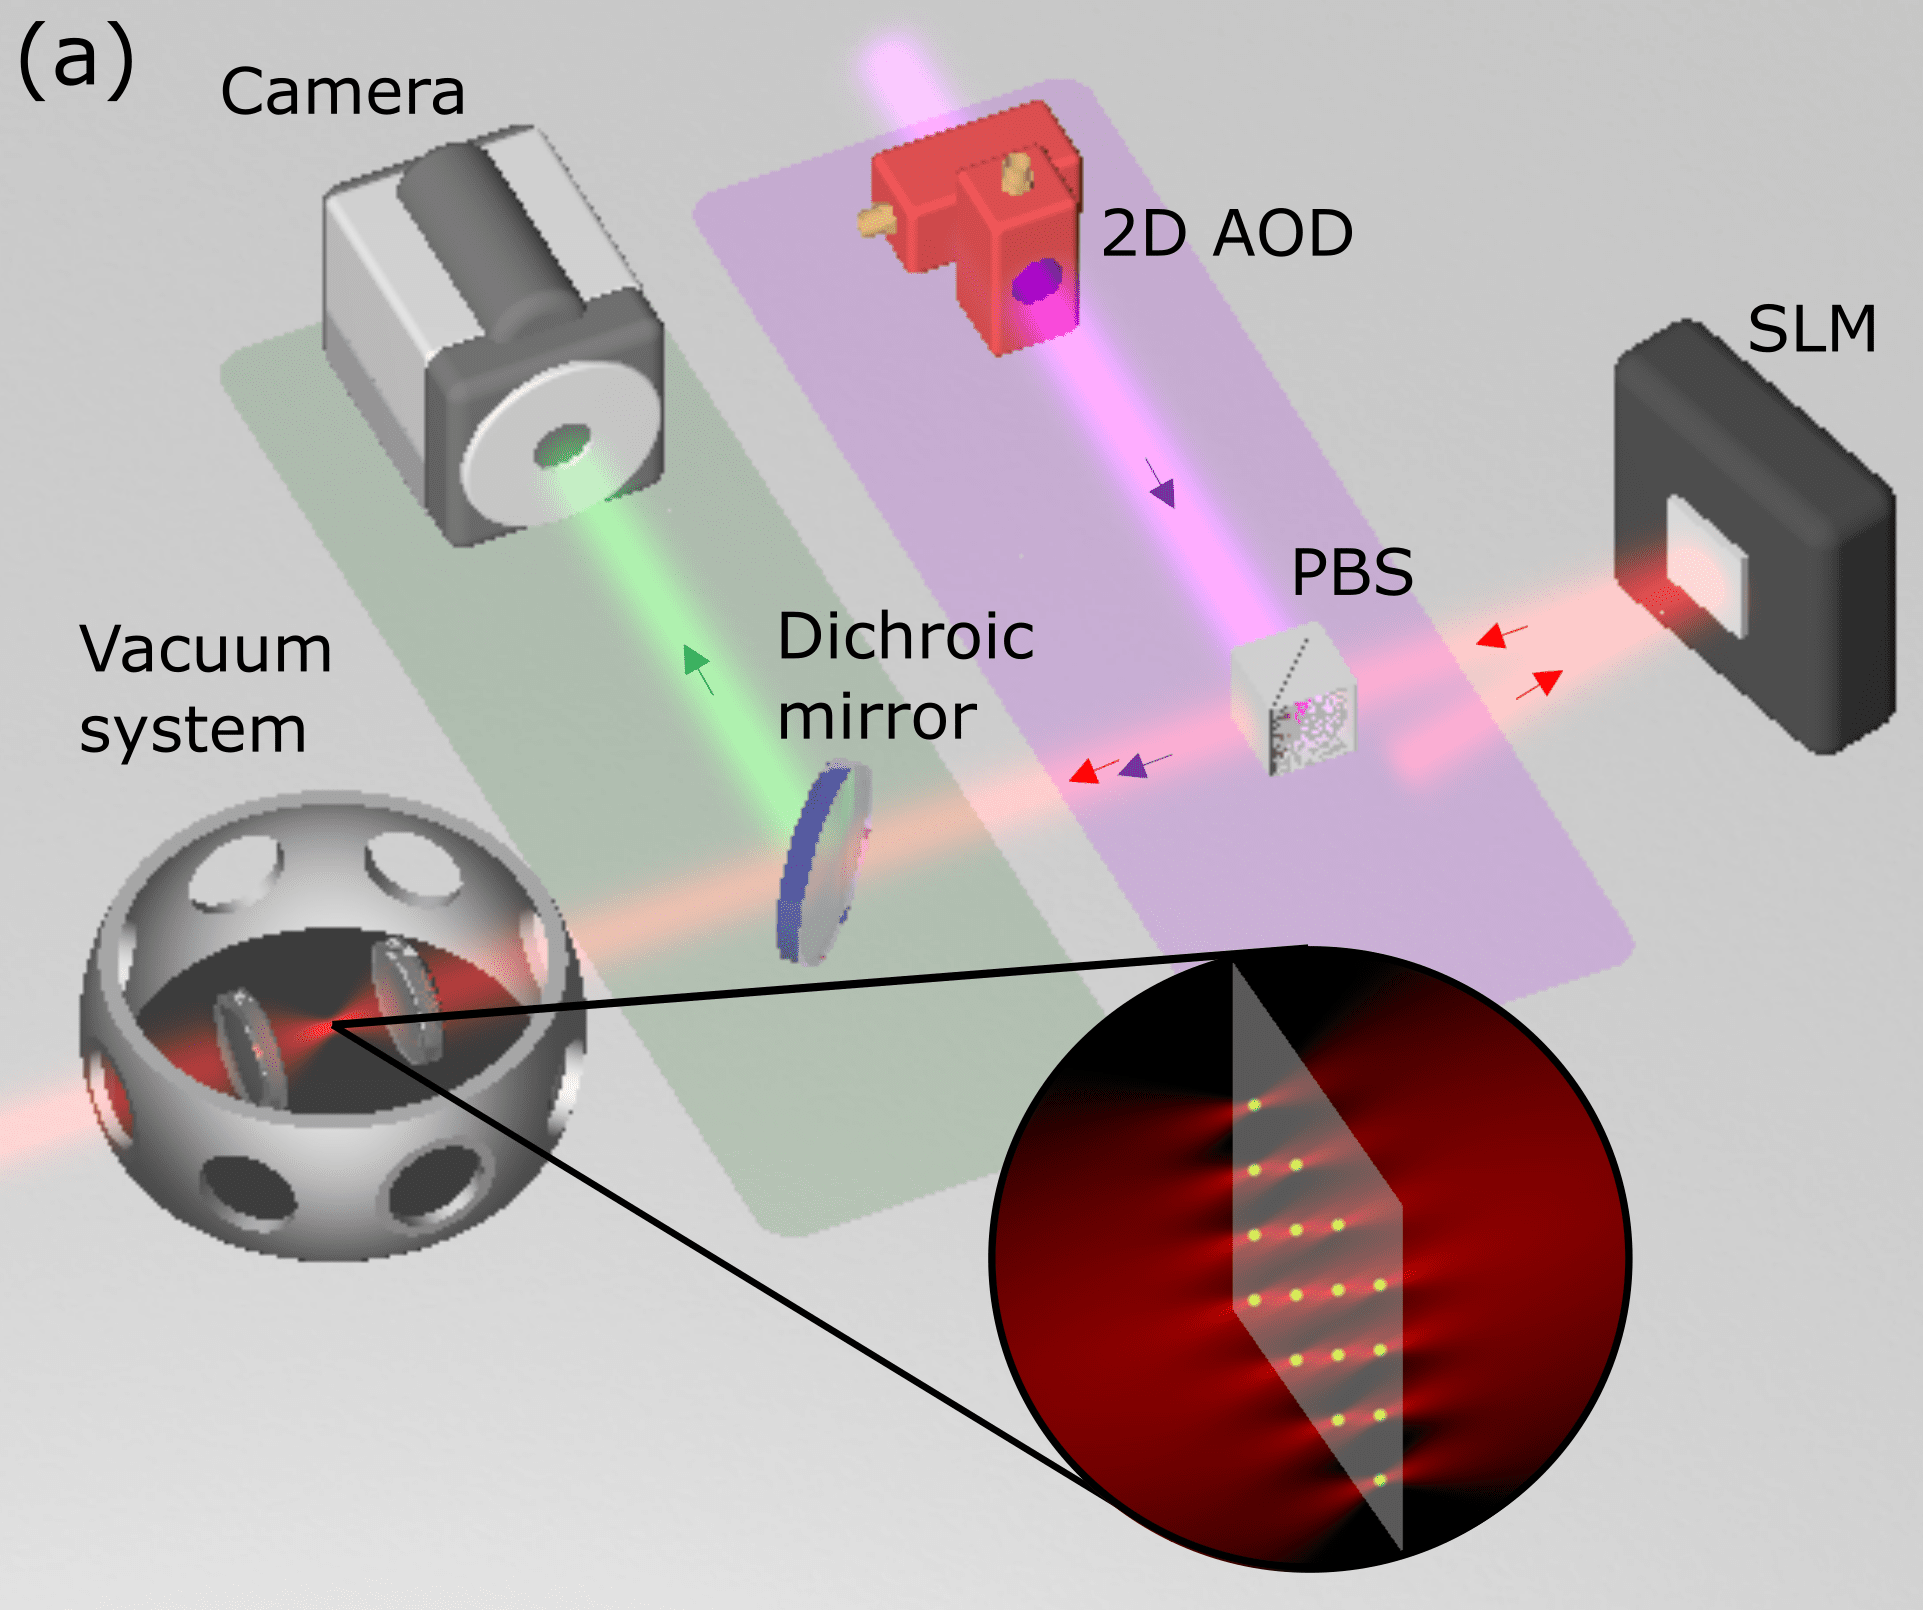
\includegraphics[width=.9\textwidth]{images/image.png}
                \caption{Overview of the main hardware components constituting a quantum processor}
            \end{figure}
        \end{column}
    \end{columns}
\end{frame}
\begin{frame}{Optical Traps and Tweezers}
  \begin{itemize}
    \item \textbf{Atom Trapping Methods}
      \begin{itemize}
        \item Optical dipole traps
        \item Optical tweezers created by lasers
      \end{itemize}
    \item \textbf{Array Configurations}
      \begin{itemize}
        \item One-, two-, or three-dimensional setups
      \end{itemize}
    \item \textbf{Dynamic Control}
      \begin{itemize}
        \item Reloading and rearrangement of atoms
        \item Enhances scalability and qubit adjustment
      \end{itemize}
  \end{itemize}
  % \includegraphics[width=0.8\textwidth]{optical_traps.pdf}
\end{frame}

\begin{frame}{Single-Qubit Gates with Rydberg Atoms}
  \begin{itemize}
    \item \textbf{Single-Qubit Operations}
      \begin{itemize}
        \item Laser pulses drive Rabi oscillations
        \item Controlled via Rabi frequency and detuning
      \end{itemize}
  \end{itemize}
  \begin{itemize}
        \item Implemented by driving Rabi oscillations between qubit states \( |0\rangle \) and \( |1\rangle \).
        \item Hamiltonian: 
        \[
            \frac{H_1(t)}{\hbar} = \frac{\Omega(t)}{2} |0\rangle\langle 1| + \frac{\Omega^*(t)}{2} |1\rangle\langle 0| - \Delta(t) |1\rangle\langle 1|
        \]
        where \( \Omega(t) \) and \( \Delta(t) \) are Rabi frequency and detuning.
        \item Single- or two-photon transitions used, with options for individual or global laser addressing.
    \end{itemize}
  % \includegraphics[width=0.8\textwidth]{laser_manipulation.pdf}
\end{frame}
\begin{frame}{Two-Qubit Gates with Rydberg Atoms}
    % \textbf{Single-Qubit Gates:}
    % \item \textbf{Multi-Qubit Gates}
    %   \begin{itemize}
    %     \item Utilize Rydberg states for entanglement
    %     \item Enable effective interactions between atoms
    % \end{itemize}
    
    \vspace{0.5cm}
    \textbf{Two-Qubit Gates via Rydberg Blockade:}
    \begin{itemize}
        \item Rydberg blockade prevents simultaneous excitation of two nearby atoms to Rydberg states (one or more electrons that have a very high principal quantum number, n).
        \item Blockade radius \( r_b \) defines the interaction range:
        \[
            r_b \simeq \left( \frac{C_6}{\hbar \Omega_r} \right)^{1/6}
        \]
        \item Enables two-qubit gates for atoms beyond nearest neighbors, increasing connectivity.
    \end{itemize}
\end{frame}
\begin{frame}{Multi-qubit gates Gates with Rydberg Atoms}
    \begin{figure}
        \centering
        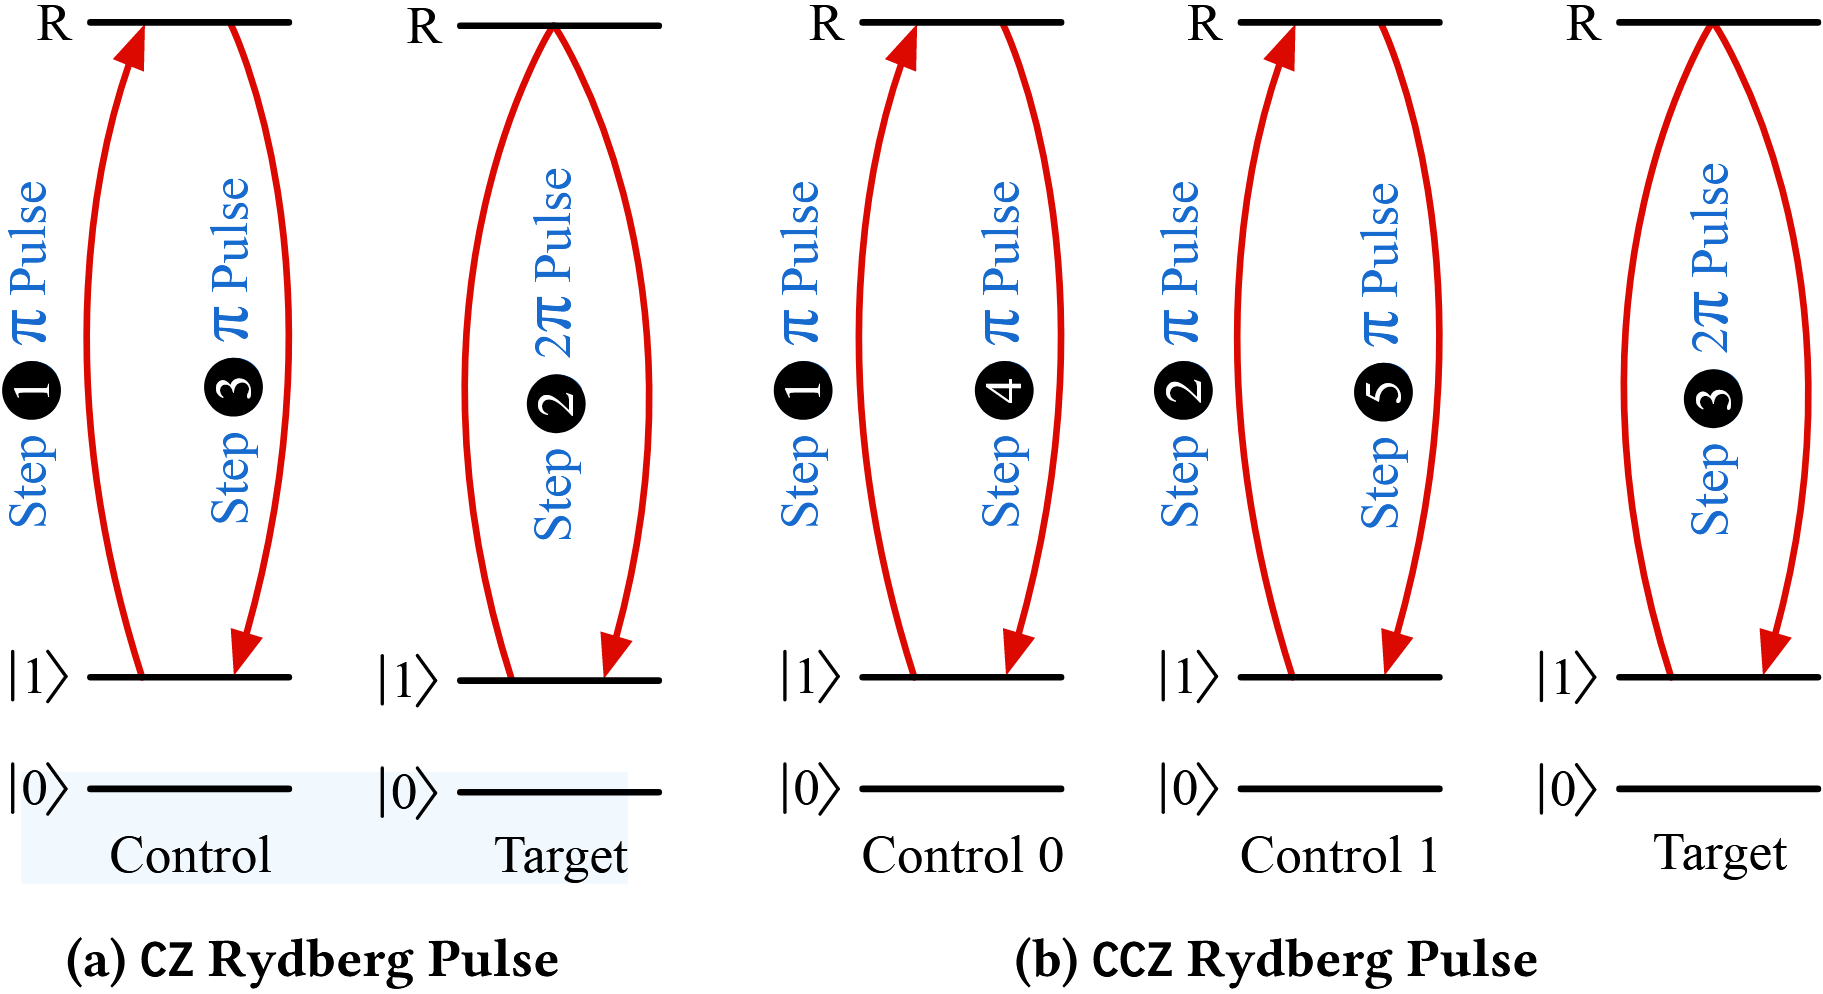
\includegraphics[width=0.8\linewidth]{images/multi-gate.png}
    \end{figure}
\end{frame}

% \begin{frame}{Shutting Atoms}

% \begin{itemize}
%     \item \textbf{Atom Shuttling in NAQC}
%     \begin{itemize}
%         \item Tweezers holding qubits can move dynamically without breaking entanglement, bypassing the need for virtual SWAP operations (3 CX gates).
%         \item Enables \textbf{flexible, dynamic qubit connectivity} by physically moving atoms.
%     \end{itemize}

%     \item \textbf{Shuttling Process}
%     \begin{itemize}
%         \item Atoms are transferred from static Spatial Light Modulator (SLM) traps to dynamic Acousto-Optic Deflector (AOD) traps.
%         \item Controlled AOD frequency ramps rearrange qubits, followed by their release back to static traps.
%     \end{itemize}

%     \item \textbf{Dynamically Field-programmable Qubit Arrays (DPQA)}
%     \begin{itemize}
%         \item A shuttling-focused processor design, avoiding a fixed grid layout.
%         \item Adds separate zones for entangling, measuring, and storing qubits, optimizing operations.
%         \item Introduces a \textbf{trade-off}: routing overhead vs. gate-based mapping.
%     \end{itemize}
% \end{itemize}

% \end{frame}
\begin{frame}{Shutting Atoms}

\begin{itemize}
    \item \textbf{Shuttling Process}
    \begin{itemize}
        \item Qubits transferred between static (SLM) and dynamic (AOD) traps.
        \item Controlled AOD frequency moves qubits, then releases to static trap.
    \end{itemize}
    \item \textbf{Dynamically Field-programmable Qubit Arrays (DPQA)}
    \begin{itemize}
        \item Shuttling-only processor design with entangling, measuring, and storage zones.
        \item Balances routing overhead and operation optimization.
    \end{itemize}
    \item \textbf{Benefits of Shuttling in NAQC}
    \begin{itemize}
        \item Dynamically moves qubits without breaking entanglement.
        \item Replaces virtual SWAP (3 CX gates) for flexible qubit connections.
    \end{itemize}
    
\end{itemize}

\end{frame}
\begin{frame}{Shuttling Process}
    \begin{columns}
        \begin{column}{.48\textwidth}
            \begin{figure}
                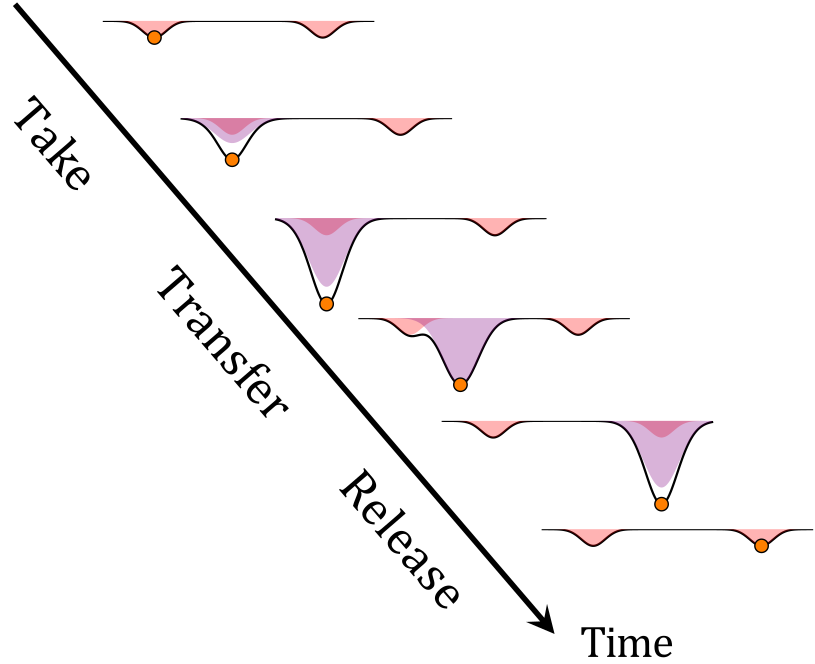
\includegraphics[width=.8\textwidth]{images/rearrange.png}
                \caption{Moving a single atom from one site to another in the register}
            \end{figure}
        \end{column}
        \begin{column}{.48\textwidth}
            \begin{figure}
                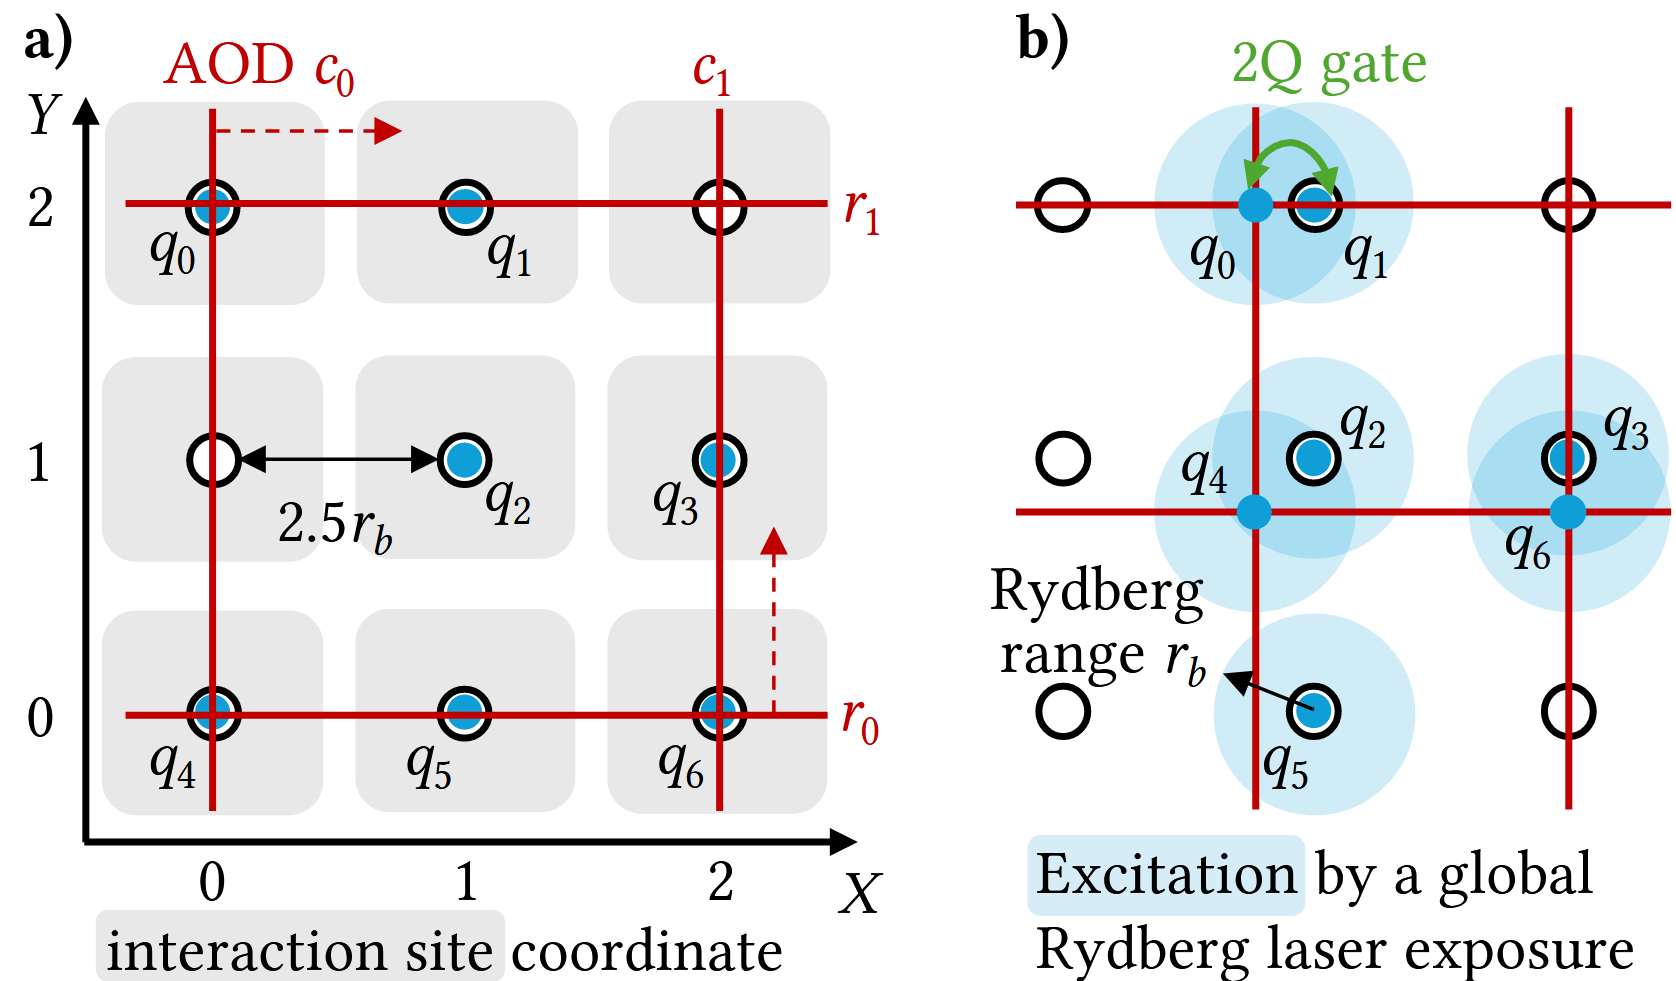
\includegraphics[width=.8\textwidth]{images/dpqa.png}
                \caption{DPQA}
            \end{figure}
        \end{column}
    \end{columns}
\end{frame}
\subsection{Scalability and Noise in Neutral Atom Devices}
\begin{frame}{Scalability Potential}
  \begin{itemize}
    \item \textbf{Flexible Arrangement}
      \begin{itemize}
        \item Atoms arranged in customizable geometries
      \end{itemize}
    \item \textbf{Long-Range Interactions}
      \begin{itemize}
        \item Rydberg blockade enables distant entanglement
      \end{itemize}
    \item \textbf{Atom Shuttling}
      \begin{itemize}
        \item Physical movement enhances connectivity
      \end{itemize}
  \end{itemize}
  % \includegraphics[width=0.8\textwidth]{scalability.pdf}
\end{frame}

\begin{frame}{Challenges in Scaling Up}
  \begin{itemize}
    \item \textbf{Cross-Talk}
      \begin{itemize}
        \item Limited precision in laser focus (Stark effect)
        \item Unintended interactions during Rydberg transitions
      \end{itemize}
    \item \textbf{Maintaining Coherence}
      \begin{itemize}
        \item Coherence times may decrease with system size
      \end{itemize}
    \item \textbf{Reliable Atom Control}
      \begin{itemize}
        \item Preventing atom loss and decoherence during trapping and shuttling
      \end{itemize}
  \end{itemize}
\end{frame}

% Slide: Comparison with Other Platforms
\begin{frame}{Differences in Noise Sources Compared to Other Platforms}
    \begin{block}{Superconducting Qubits}
        \begin{itemize}
            \item Sensitive to electromagnetic noise and material defects
            \item Decoherence due to charge and flux noise
        \end{itemize}
    \end{block}
    \begin{block}{Trapped Ion Qubits}
        \begin{itemize}
            \item Susceptible to electric field fluctuations
            \item Motional heating and laser noise
        \end{itemize}
    \end{block}
    \begin{block}{Photonic Qubits}
        \begin{itemize}
            \item Affected by atom loss and detector inefficiencies
            \item Immune to thermal noise affecting matter-based qubits
        \end{itemize}
    \end{block}
\end{frame}

% Slide: Common Noise Sources in Neutral Atom QC
% \begin{frame}{Common Noise Sources in Neutral Atom Quantum Computing}
%     \begin{enumerate}
%         \item \textbf{Laser Noise}
%         \begin{itemize}
%             \item Intensity fluctuations affect trap depth
%             \item Frequency and phase noise cause dephasing
%         \end{itemize}
%         \item \textbf{Atom Loss}
%         \begin{itemize}
%             \item Collisions with background gas
%             \item Photon scattering leading to heating
%         \end{itemize}
%         \item \textbf{Decoherence Mechanisms}
%         \begin{itemize}
%             \item Spontaneous emission
%             \item Interactions with blackbody radiation
%         \end{itemize}
%         \item \textbf{Motional Decoherence}
%         \begin{itemize}
%             \item Residual thermal motion
%             \item Fluctuations in trapping potential
%         \end{itemize}
%         \item \textbf{Control Field Errors}
%         \begin{itemize}
%             \item Laser beam imperfections
%             \item Timing jitter in control pulses
%         \end{itemize}
%         \item \textbf{Rydberg State Decay}
%         \begin{itemize}
%             \item Finite lifetimes due to spontaneous emission
%             \item State mixing from external fields
%         \end{itemize}
%     \end{enumerate}
% \end{frame}
\begin{frame}{Common Noise Sources in Neutral Atom Quantum Computing}
    \begin{itemize}
        \item \textbf{Laser Noise:} Intensity fluctuations, frequency/phase noise
        \item \textbf{Atom Loss:} Background gas collisions, photon scattering
        \item \textbf{Decoherence:} Spontaneous emission, blackbody radiation
        \item \textbf{Motional Decoherence:} Thermal motion, trap fluctuations
        \item \textbf{Control Errors:} Beam imperfections, timing jitter
        \item \textbf{Rydberg Decay:} Finite lifetimes, state mixing
    \end{itemize}
\end{frame}

% Slide: Mitigation Strategies
% \begin{frame}{Mitigation Strategies}
%     \begin{itemize}
%         \item \textbf{Laser Stabilization}
%         \begin{itemize}
%             \item High-quality lasers with active stabilization
%         \end{itemize}
%         \item \textbf{Vacuum Improvements}
%         \begin{itemize}
%             \item Enhanced vacuum conditions to reduce collisions
%         \end{itemize}
%         \item \textbf{Cooling Techniques}
%         \begin{itemize}
%             \item Raman sideband cooling to reduce atomic motion
%         \end{itemize}
%         \item \textbf{Error Correction Codes}
%         \begin{itemize}
%             \item Implement quantum error correction protocols
%         \end{itemize}
%         \item \textbf{Optimal Control}
%         \begin{itemize}
%             \item Design robust control pulses against imperfections
%         \end{itemize}
%     \end{itemize}
% \end{frame}

\begin{frame}{Mitigation Strategies}
    \begin{itemize}
        \item \textbf{Laser Stabilization:} High-quality lasers with active stabilization
        \item \textbf{Vacuum Improvements:} Enhanced vacuum conditions
        \item \textbf{Cooling Techniques:} Raman sideband cooling
        \item \textbf{Error Correction:} Quantum error correction protocols
        \item \textbf{Optimal Control:} Robust control pulse design
    \end{itemize}
\end{frame}




\section{Related Work}
\begin{frame}[fragile]
\frametitle{Key Compilation Subroutines during Compilation}
\begin{itemize}
    \item \textbf{Platform-independent Compilation:}General optimizations, e.g., loop unrolling and gate commutation.
    \item \textbf{Platform-dependent Compilation:}Adapts quantum circuits to specific hardware constraints and capabilities.
    \item \textbf{Hardware-dependent Compilation:}Translates abstract operations into hardware-executable instructions.
\end{itemize}
\end{frame}
\begin{frame}{primary objectives}
\begin{itemize}
    \item \textbf{Synthesis:} Decompose gates into native hardware-compatible operations.
    \item \textbf{Mapping:} Assign logical qubits to physical qubits, introducing SWAP/MOVE operations.
    \item \textbf{Scheduling:} Optimize gate execution timing to maximize parallelism and minimize errors.
\end{itemize}
attention:
\begin{itemize}
    \item NAQC-specific capabilities like atom shuttling and Rydberg interactions affect all steps.
    \item Compilation steps are often optimized collectively for hardware constraints. 
\end{itemize}
\end{frame}

\begin{frame}
\frametitle{SC Compilation Challenges for NAQC}
\begin{itemize}
    \item \textbf{Synthesis:} 
    SC only supports one- and two-qubit gates, making multi-qubit gates challenging.
    \item \textbf{Mapping:} 
    SC relies on virtual swaps for connectivity, while NAQC defines coupling using \(r_{\text{int}}\).
    \item \textbf{Scheduling:} 
    NAQC adds constraints from the restriction radius, requiring tailored adjustments.
\end{itemize}
\end{frame}


\begin{frame}{Overview of Related Work on NAQC Compilation}
    \begin{itemize}
        \item Neutral atom quantum computing (NAQC) introduces unique challenges and capabilities.
        \item Related works address these through distinct themes:
        \begin{itemize}
            \item Long-range interactions
            \item Multi-qubit gates
            \item Shuttling operations
            \item Adaptation of superconducting (SC) compilers
        \end{itemize}
    \end{itemize}
\end{frame}

\begin{frame}{Long-range Compilers}
    \textbf{Two Major Implementations:}
    \vspace{0.5em}
    
    \begin{columns}
        \column{0.5\textwidth}
        \textbf{Baker et al. [33]}
        \begin{itemize}
            \item Focus: Mapping \& atom loss
            \item Features parallel SWAP execution
            \item Uses look-ahead schemes
        \end{itemize}
        
        \column{0.5\textwidth}
        \textbf{Q-Tetris [28]}
        \begin{itemize}
            \item Greedy heuristic algorithm
            \item Monte Carlo tree search
            \item Time-efficient optimization
        \end{itemize}
    \end{columns}
\end{frame}

\begin{frame}{Multi-qubit Compiler}
    \textbf{Geyser [29, 115]}
    \begin{itemize}
        \item Novel approach to multi-qubit operations
        \item Key features:
        \begin{itemize}
            \item Composes Toffoli gates from two-qubit gates
            \item Uses Qiskit for mapping
            \item Optimizes laser pulse count
        \end{itemize}
        \item Evaluation metric: laser pulse count vs. gate count
    \end{itemize}
\end{frame}

\begin{frame}{Shuttling Compilers (1/2)}
    \textbf{First Generation:}
    \begin{itemize}
        \item \textbf{Brandhofer et al. [31]}
        \begin{itemize}
            \item 1D atom displacements
            \item SMT solver optimization
        \end{itemize}
        \item \textbf{Tan et al. [111, 116]}
        \begin{itemize}
            \item DPQA architecture focus
            \item Visual movement animations
            \item 2D shuttling capability
        \end{itemize}
        \item \textbf{Schmid et al. [36]}
        \begin{itemize}
            \item Hybrid compilation scheme
            \item SABRE-based heuristic
            \item Comprehensive capability support
        \end{itemize}
    \end{itemize}
\end{frame}

\begin{frame}{Future Challenges}
    \begin{itemize}
        \item Synthesis improvements needed for:
        \begin{itemize}
            \item General quantum algorithms
            \item Multi-qubit gate integration
        \end{itemize}
        \item Integration of multiple capabilities
        \item Hardware-dependent error analysis
        \item Platform accessibility improvement
    \end{itemize}
    \vspace{1em}
    \centering
    Goal: Full exploitation of NAQC platform potential
\end{frame}

\section{Our work}

\subsection{DasAtom Transformation Method}

\begin{frame}{Subgraph Isomorphism in Quantum Circuit Mapping}
  \begin{itemize}
    \item \textbf{DasAtom} uses subgraph isomorphism to map quantum circuits onto neutral atom (NA) architectures.
    \item Ensures each gate in a subcircuit is directly executable.
    \item Embedding interaction graphs onto the NA grid enhances fidelity and efficiency.
  \end{itemize}

  % Uncomment to include an illustrative figure
  % \begin{figure}
  % \centering
  % \includegraphics[width=0.8\linewidth]{interaction_graph_example.png}
  % \caption{Mapping the interaction graph onto the NA architecture using subgraph isomorphism.}
  % \end{figure}
\end{frame}

\begin{frame}{DasAtom Algorithm Overview}
  The algorithm operates in four main steps:

  \begin{enumerate}
    \item \textbf{Partitioning}
      \begin{itemize}
        \item Divide the quantum circuit into CZ layers and subcircuits.
        \item Ensure each layer is fully contained within a subcircuit.
      \end{itemize}
    \item \textbf{Embedding}
      \begin{itemize}
        \item Find optimal qubit mappings for each subcircuit onto the NA grid.
      \end{itemize}
    \item \textbf{Parallel Execution}
      \begin{itemize}
        \item Execute gates in each subcircuit in parallel.
        \item Consider blockade radius constraints of the NA architecture.
      \end{itemize}
    \item \textbf{Routing via Atom Shuttling}
      \begin{itemize}
        \item Use atom shuttling to transition between different qubit mappings.
        \item Enable efficient, high-fidelity transformations.
      \end{itemize}
  \end{enumerate}

  % Uncomment to include a flowchart of the algorithm
  % \begin{figure}
  % \centering
  % \includegraphics[width=0.8\linewidth]{dasatom_flowchart.png}
  % \caption{Flowchart of the DasAtom transformation framework.}
  % \end{figure}
\end{frame}
\begin{frame}{Running example}
    \centering
  \scalebox{0.5}{% \documentclass{standalone}
% \usepackage{tikz}
% \usetikzlibrary{patterns}
% \begin{document}
\begin{tikzpicture}
    \definecolor{lightgray}{rgb}{0.8,0.8,0.8}
    \definecolor{darkgreen}{rgb}{0  ,0.5,0  }
    \tikzset{
        unuseNode/.style={
            circle,
            draw=blue,
            dashed, % Dashed outline
            % fill=red, % Solid fill color
            % pattern=vertical lines, % Pattern type
            minimum size=8pt,
            inner sep=0pt
        },
        useNode/.style={circle, draw=none, fill=blue,minimum size=8pt, inner sep=0pt},
        fontNode1/.style={above right, font=\Large },
        fontNode2/.style={right, midway,font=\small}
    }
    % Set the color and style of the grid lines
    \draw[lightgray, dashed, xstep =3, ystep =3] (0,0) grid (6,6);
    
    % Draw the x and y axis arrows
    \draw[->, thick] (-0.2,-0.2) -- (6.4,-0.2) node[below] {x};
    \draw[->, thick] (-0.2,-0.2) -- (-0.2,6.4) node[left] {y};

    % Draw the bevels (diagonals in each grid square)
    \foreach \x in {0,3} {
        \foreach \y in {0,3} {
            \draw[lightgray, dashed] (\x,\y) -- (\x+3,\y+3); % Diagonal from bottom-left to top-right
            \draw[lightgray, dashed] (\x+3,\y) -- (\x,\y+3); % Diagonal from bottom-right to top-left
        }
    }
    
    % Add labels for the x-axis
    \foreach \x in {0,1,2} {
        \node[below] at ({3*\x}, -0.2) {\small \x};
    }

    % Add labels for the y-axis
    \foreach \y in {0,1,2} {
        \node[left] at (-0.2, {3*\y}) {\small \y};
    }

    \node[useNode] (q0) at (0,6) {};
    \node[fontNode1] at (q0) {$q0$};
    \node[useNode] (q1) at (3,0) {};
    \node[fontNode1] at (q1) {$q1$};
    \node[useNode] (q2) at (0,0) {};
    \node[fontNode1] at (q2) {$q2$};
    \node[useNode] (q3) at (3,3) {};
    \node[fontNode1] at (q3) {$q3$};
    \node[useNode] (q4) at (0,3) {};
    \node[fontNode1] at (q4) {$q4$};
\end{tikzpicture}
% \end{document}
}
  \scalebox{0.5}{% \documentclass{standalone}
% \usepackage{tikz}
% \usetikzlibrary{patterns}
% \begin{document}
\begin{tikzpicture}
    \definecolor{lightgray}{rgb}{0.8,0.8,0.8}
    \definecolor{darkgreen}{rgb}{0  ,0.5,0  }
    \tikzset{
        unuseNode/.style={
            circle,
            draw=blue,
            dashed, % Dashed outline
            % fill=red, % Solid fill color
            % pattern=vertical lines, % Pattern type
            minimum size=12pt,
            inner sep=0pt
        },
        useNode/.style={circle, draw=black, minimum size=8pt, inner sep=2pt},
        fontNode1/.style={above right, font=\Large },
        fontNode2/.style={right, midway,font=\small}
    }


    % \node[useNode] (q0) at (0,6) {};
    % \node[fontNode1] at (q0) {$q0$};
    % \node[useNode] (q1) at (3,0) {};
    % \node[fontNode1] at (q1) {$q1$};
    % \node[useNode] (q2) at (0,0) {};
    % \node[fontNode1] at (q2) {$q2$};
    % \node[useNode] (q3) at (3,3) {};
    % \node[fontNode1] at (q3) {$q3$};
    % \node[useNode] (q4) at (0,3) {};
    % \node[fontNode1] at (q4) {$q4$};
    \node[useNode] (q0) at (0,6) {$q0$};
    \node[useNode] (q1) at (3,0) {$q1$};
    \node[useNode] (q2) at (0,0) {$q2$};
    \node[useNode] (q3) at (3,3) {$q3$};
    \node[useNode] (q4) at (0,3) {$q4$};

    \draw[-,line width = 0.3mm] (q0) -- (q4) node[fontNode2] {};
    \draw[-,line width = 0.3mm] (q0) -- (q3) node[fontNode2] {};
    \draw[-,line width = 0.3mm] (q4) -- (q3) node[fontNode2] {};
    \draw[-,line width = 0.3mm] (q4) -- (q2) node[fontNode2] {};
    \draw[-,line width = 0.3mm] (q4) -- (q1) node[fontNode2] {};
    \draw[-,line width = 0.3mm] (q3) -- (q2) node[fontNode2] {};
    \draw[-,line width = 0.3mm] (q1) -- (q3) node[fontNode2] {};
    \draw[-,line width = 0.3mm] (q1) -- (q2) node[fontNode2] {};
\end{tikzpicture}
% \end{document}
}
  \scalebox{0.5}{% \documentclass{standalone}
% \usepackage{tikz}
% \usetikzlibrary{patterns}
% \begin{document}
\begin{tikzpicture}
    \definecolor{lightgray}{rgb}{0.8,0.8,0.8}
    \definecolor{darkgreen}{rgb}{0  ,0.5,0  }
    \tikzset{
        unuseNode/.style={
            circle,
            draw=blue,
            dashed, % Dashed outline
            % fill=red, % Solid fill color
            % pattern=vertical lines, % Pattern type
            minimum size=8pt,
            inner sep=0pt
        },
        useNode/.style={circle, draw=none, fill=blue, minimum size=8pt, inner sep=0pt},
        fontNode1/.style={above right, font=\Large },
        fontNode2/.style={right, midway,font=\small}
    }
    % Set the color and style of the grid lines
    \draw[lightgray, dashed, xstep =3, ystep =3] (0,0) grid (6,6);
    
    % Draw the x and y axis arrows
    \draw[->, thick] (-0.2,-0.2) -- (6.4,-0.2) node[below] {x};
    \draw[->, thick] (-0.2,-0.2) -- (-0.2,6.4) node[left] {y};

    % Draw the bevels (diagonals in each grid square)
    \foreach \x in {0,3} {
        \foreach \y in {0,3} {
            \draw[lightgray, dashed] (\x,\y) -- (\x+3,\y+3); % Diagonal from bottom-left to top-right
            \draw[lightgray, dashed] (\x+3,\y) -- (\x,\y+3); % Diagonal from bottom-right to top-left
        }
    }
    
    % Add labels for the x-axis
    \foreach \x in {0,1,2} {
        \node[below] at ({3*\x}, -0.2) {\small \x};
    }

    % Add labels for the y-axis
    \foreach \y in {0,1,2} {
        \node[left] at (-0.2, {3*\y}) {\small \y};
    }

    \node[useNode] (q0) at (0,3) {};
    \node[fontNode1] at (q0) {$q0$};
    \node[useNode] (q1) at (0,6) {};
    \node[fontNode1] at (q1) {$q1$};
    \node[useNode] (q2) at (0,0) {};
    \node[fontNode1] at (q2) {$q2$};
    \node[useNode] (q3) at (3,3) {};
    \node[fontNode1] at (q3) {$q3$};
    \node[useNode] (q4) at (3,0) {};
    \node[fontNode1] at (q4) {$q4$};
\end{tikzpicture}
% \end{document}}
  \scalebox{0.5}{% \documentclass{standalone}
% \usepackage{tikz}
% \usetikzlibrary{patterns}
% \begin{document}
\begin{tikzpicture}
    \definecolor{lightgray}{rgb}{0.8,0.8,0.8}
    \definecolor{darkgreen}{rgb}{0  ,0.5,0  }
    \tikzset{
        unuseNode/.style={
            circle,
            draw=blue,
            dashed, % Dashed outline
            % fill=red, % Solid fill color
            % pattern=vertical lines, % Pattern type
            minimum size=8pt,
            inner sep=0pt
        },
        useNode/.style={circle, draw=black, minimum size=8pt, inner sep=2pt},
        fontNode1/.style={above right, font=\Large },
        fontNode2/.style={right, midway,font=\small}
    }


    % \node[useNode] (q0) at (0,6) {};
    % \node[fontNode1] at (q0) {$q0$};
    % \node[useNode] (q1) at (3,0) {};
    % \node[fontNode1] at (q1) {$q1$};
    % \node[useNode] (q2) at (0,0) {};
    % \node[fontNode1] at (q2) {$q2$};
    % \node[useNode] (q3) at (3,3) {};
    % \node[fontNode1] at (q3) {$q3$};
    % \node[useNode] (q4) at (0,3) {};
    % \node[fontNode1] at (q4) {$q4$};
    \node[useNode] (q0) at (0,3) {$q0$};
    \node[useNode] (q1) at (0,6) {$q1$};
    \node[useNode] (q2) at (0,0) {$q2$};
    \node[useNode] (q3) at (3,3) {$q3$};
    \node[useNode] (q4) at (3,0) {$q4$};

    \draw[-,line width = 0.3mm] (q0) -- (q1) node[fontNode2] {};
    \draw[-,line width = 0.3mm] (q0) -- (q2) node[fontNode2] {};
\end{tikzpicture}
% \end{document}
}
\end{frame}
\subsection{Comparative Analysis}

\begin{frame}{Performance Comparison with Existing Methods}
  \begin{itemize}
    \item \textbf{Fidelity Improvements}
      \begin{itemize}
        \item 414x over Enola
        \item 10.6x over Tetris
        \item 16.1x over Atomique
        \item Evaluated on a 30-qubit Quantum Fourier Transform (QFT) circuit
      \end{itemize}
    \item \textbf{Reduced Compilation Time}
      \begin{itemize}
        \item Significantly shorter runtimes for larger circuits
        \item Outperforms existing methods on complex topologies
      \end{itemize}
  \end{itemize}

  % Uncomment to include a comparative performance chart
  % \begin{figure}
  % \centering
  % \includegraphics[width=\linewidth]{comparison_chart.png}
  % \caption{Performance comparison of DasAtom with existing methods.}
  % \end{figure}
\end{frame}
\begin{frame}{Ablation studies on QFT-20}
\begin{figure}
    \centering
    \pgfplotsset{
        F_CZ_axis/.style={
            xlabel={$f_\text{cz}$},
            ylabel={fidelity},
            xtick={0.95,0.96,0.98,0.99,0.999},
            xticklabel style={
                /pgf/number format/fixed,
                /pgf/number format/precision=3,
                rotate=45,
                anchor=east
            },
            width = 8cm,
            height = 6cm,
            % legend pos=north west,
            grid=both,
            % legend entries={DasAtom, Tetris, Enola, Atomique},
            mark repeat=1                   % Controls how often markers are placed
            ,
            xlabel style = {font =\Large},
            ylabel style = {font =\Large},
        },
        F_atom_trans_axis/.style={
            xlabel={$f_\text{trans}$},
            ylabel={fidelity},
            xtick={0.991,0.993,0.995,0.997,0.999,1},
            xticklabel style={
                /pgf/number format/fixed,
                /pgf/number format/precision=3,
                rotate=45,
                anchor=east
            },
            width = 8cm,
            height = 6cm,
            grid=both,
            mark repeat=1,
            xlabel style = {font =\Large},
            ylabel style = {font =\Large},
            scaled y ticks=false
        },
        T2_axis/.style={
            xlabel={$T_2$},
            ylabel={fidelity},
            xtick={0.15, 1.5, 5, 10, 15},
            xticklabel style={
                /pgf/number format/fixed,
                /pgf/number format/precision=3,
                rotate=45,
                anchor=east
            },
            width = 8cm,
            height = 6cm,
            % legend pos=north west,
            grid=both,
            % legend entries={DasAtom, Tetris, Enola, Atomique},
            mark repeat=1                    % Controls how often markers are placed
            ,
            xlabel style = {font =\Large},
            ylabel style = {font =\Large},
            ytick={0, 0.05,0.1},
            yticklabel style={
            /pgf/number format/fixed,
            /pgf/number format/precision=2
            },
            scaled y ticks=false
        },
        dis_axis/.style={
            xlabel={Atom distance},
            ylabel={fidelity},
            xtick={1, 3, 5, 7, 9, 11, 13, 15, 17, 20},
            xticklabel style={
                /pgf/number format/fixed,
                /pgf/number format/precision=3,
                rotate=45,
                anchor=east
            },
            width = 8cm,
            height = 6cm,
            grid=both,
            mark repeat=1,
            xlabel style = {font =\Large},
            ylabel style = {font =\Large}, 
            ytick={0, 0.05,0.1},
            yticklabel style={
            /pgf/number format/fixed,
            /pgf/number format/precision=2
            },
            scaled y ticks=false
        }
    }
    \begin{minipage}[b]{0.45\textwidth}
            \centering
            \scalebox{0.5}{% TikZ code for QFT Benchmark
\begin{tikzpicture}
\begin{axis}[F_atom_trans_axis,ymode=log,
legend entries={DasAtom,Tetris, Enola, Atomique},
legend pos=south east,
]
\addplot [DasAtomStyle]
table {%
0.991	0.001651072
0.992	0.002657727
0.993	0.004276086
0.994	0.006876612
0.995	0.011053383
0.996	0.017758605
0.997	0.028517788
0.998	0.045773762
0.999	0.073436431
1	      0.1177609
};

\addplot [TetrisStyle]
table {%
0.991	0.023751235
0.992	0.023751235
0.993	0.023751235
0.994	0.023751235
0.995	0.023751235
0.996	0.023751235
0.997	0.023751235
0.998	0.023751235
0.999	0.023751235
1	0.023751235
};

\addplot [EnolaStyle]
table {%
0.991	6.71372e-09
0.992	3.49591e-08
0.993	1.81734e-07
0.994	9.43169e-07
0.995	4.8868e-06
0.996	2.5278e-05
0.997	0.00013054
0.998	0.000673024
0.999	0.003464204
1	0.017801835
};

\addplot [AtomiqueStyle]
table {%
0.991	0.048179571
0.992	0.048179571
0.993	0.048179571
0.994	0.048179571
0.995	0.048179571
0.996	0.048179571
0.997	0.048179571
0.998	0.048179571
0.999	0.048179571
1	0.048179571
};

\end{axis}
% \node[anchor=south east] at (6.5, 0)  {
% \begin{tikzpicture}
% Define the block size
\draw[gray!40,fill=gray!10] (-1.4em, 0.2em) rectangle (7em, 5.2em);

% Legend entry for DasAtom with line and marker
\node at (0, 4em) {
    \tikz \draw[DasAtomStyle] (0, 0.5em) -- (2em, 0.5em);
};
\node[anchor=west] at (2.5em, 4em) {DasAtom};

% Legend entry for Tetris with line and marker
\node at (0, 3em) {
    \tikz \draw[TetrisStyle] (0, 0.5em) -- (2em, 0.5em);
};
\node[anchor=west] at (2.5em, 3em) {Tetris};

% Legend entry for Enola with line and marker
\node at (0, 2em) {
    \tikz \draw[EnolaStyle] (0, 0.5em) -- (2em, 0.5em);
};
\node[anchor=west] at (2.5em, 2em) {Enola};

% Legend entry for Atomique with line and marker
\node at (0, 1em) {
    \tikz \draw[AtomiqueStyle] (0, 0.5em) -- (2em, 0.5em);
};
\node[anchor=west] at (2.5em, 1em) {Atomique};

\end{tikzpicture}

% };
\end{tikzpicture}
}
            % \caption*{$f_{\text{trans}}$}
        \end{minipage}
        \hfill
        \begin{minipage}[b]{0.45\textwidth}
            \centering
            \scalebox{0.5}{% TikZ code for QFT Benchmark
\begin{tikzpicture}
\begin{axis}[F_CZ_axis,ymode=log]
\addplot [DasAtomStyle]
table {%
0.95 6.764195935658048e-10
0.96 4.951577227488511e-08
0.97 3.4669618269011044e-06
0.98 0.00023239621186436929
0.99 0.014926837183020377
0.991 0.02258064534281901
0.993 0.051609528785428925
0.995 0.11776090008372139
0.997 0.2682581458421339
0.998 0.4046317325127107
0.999 0.6100819602511983
0.9999 0.8825331888319055
};

\addplot [TetrisStyle]
table {%
0.95 2.407007884506807e-17
0.96 5.943028526994131e-14
0.97 1.353261511225944e-10
0.98 2.846560600769755e-07
0.99 0.0005540170585716745
0.991 0.0011765603630107997
0.993 0.005294285348299142
0.995 0.02375123538372682
0.997 0.10623217367012125
0.998 0.22441494097715448
0.999 0.47372050543212835
0.9999 0.9274018950907676
};

\addplot [EnolaStyle]
table {%
0.95 1.0225388803239163e-10
0.96 7.485265480472717e-09
0.97 5.240982517843539e-07
0.98 3.5131176644159965e-05
0.99 0.0022564797834198434
0.991 0.0034135007361508897
0.993 0.007801777222345272
0.995 0.017801834846735642
0.997 0.040552400713463374
0.998 0.061167902680929975
0.999 0.0922256733061934
0.9999 0.13341193947379063
};

\addplot [AtomiqueStyle]
table {%
0.95 1.7223026292342555e-11
0.96 2.363167511628847e-09
0.97 3.081272329875911e-07
0.98 3.821822864242171e-05
0.99 0.004513946834858784
0.991 0.0072549193160830455
0.993 0.018713790861195394
0.995 0.04817957107394073
0.997 0.12380534231393599
0.998 0.19832131064066677
0.999 0.3175370787103337
0.9999 0.48484410267478034
};

\end{axis}

% Overlay subplot for zoom effect
    \begin{axis}[
        at={(4cm, 2.3cm)}, % Position of the subplot over the original plot
        anchor=north west, % Anchoring point to position the overlay precisely
        width=4cm, % Width of the zoom-in subplot
        height=3cm, % Height of the zoom-in subplot
        % domain=0.99:0.9999, % Define the range for zooming in
        xtick={0.998,0.999,0.9999},
        xticklabel style={
                font=\footnotesize,
                /pgf/number format/fixed,
                /pgf/number format/precision=4,
                rotate=45,
                anchor=east
            },
        % ymode=log,
        ytick = {0, 0.4, 0.7, 1},
        axis background/.style={fill=white}, % Make sure it covers original plot clearly
    ]
    \addplot [DasAtomStyle]
table {%
0.998 0.4046317325127107
0.999 0.6100819602511983
0.9999 0.8825331888319055
};

\addplot [TetrisStyle]
table {%
0.998 0.22441494097715448
0.999 0.47372050543212835
0.9999 0.9274018950907676
};

\addplot [EnolaStyle]
table {%
0.998 0.061167902680929975
0.999 0.0922256733061934
0.9999 0.13341193947379063
};

\addplot [AtomiqueStyle]
table {%
0.998 0.19832131064066677
0.999 0.3175370787103337
0.9999 0.48484410267478034
};
    \end{axis}
\end{tikzpicture}
}
            % \caption*{$f_{\text{cz}}$}
        \end{minipage}

        \vspace{0.5cm}

        \begin{minipage}[b]{0.45\textwidth}
            \centering
            \scalebox{0.5}{% TikZ code for QFT Benchmark
\begin{tikzpicture}
\begin{axis}[T2_axis]
\addplot [DasAtomStyle]
table {%
0.15	0.055315038
0.5	0.099558223
1	0.112919806
1.5	0.1177609
5	0.124889092
10	0.126471831
15	0.127003856
};

\addplot [TetrisStyle]
table {%
0.15	0.023588369
0.5	0.023714946
1	0.023742158
1.5	0.023751235
5	0.02376395
10	0.023766675
15	0.023767584
};

\addplot [EnolaStyle]
table {%
0.15	3.44731e-10
0.5	0.000343928
1	0.006636905
1.5	0.017801835
5	0.070853875
10	0.095260609
15	0.105138862
};

\addplot [AtomiqueStyle]
table {%
0.15	0.000108892
0.5	0.012442077
1	0.034345546
1.5	0.048179571
5	0.077384226
10	0.085654503
15	0.088603208
};

\end{axis}
\end{tikzpicture}
}
            % \caption*{$T_2$ (s)}
        \end{minipage}
        \hfill
        \begin{minipage}[b]{0.45\textwidth}
            \centering
            \scalebox{0.5}{% TikZ code for QFT Benchmark
\begin{tikzpicture}
\begin{axis}[dis_axis]
\addplot [DasAtomStyle]
table {%
1	0.11238292
2	0.111953559
3	0.111525838
4	0.111099752
5	0.110675294
6	0.110252457
7	0.109831236
8	0.109411624
9	0.108993615
10	0.108577203
11	0.108162382
12	0.107749146
13	0.107337488
14	0.106927404
15	0.106518886
16	0.106111929
17	0.105706526
18	0.105302673
19	0.104900362
20	0.104499588
};

\addplot [TetrisStyle]
table {%
1	0.023751235
2	0.023751235
3	0.023751235
4	0.023751235
5	0.023751235
6	0.023751235
7	0.023751235
8	0.023751235
9	0.023751235
10	0.023751235
11	0.023751235
12	0.023751235
13	0.023751235
14	0.023751235
15	0.023751235
16	0.023751235
17	0.023751235
18	0.023751235
19	0.023751235
20	0.023751235
};

\addplot [EnolaStyle]
table {%
1	0.052363273
2	0.044819981
3	0.039777254
4	0.035969491
5	0.032917995
6	0.030382667
7	0.028223905
8	0.026352635
9	0.024708239
10	0.023247461
11	0.021938285
12	0.020756318
13	0.01968253
14	0.018701784
15	0.017801835
16	0.016972636
17	0.016205846
18	0.015494459
19	0.014832542
20	0.01421502
};

\addplot [AtomiqueStyle]
table {%
1	0.051063551
2	0.049600605
3	0.048179571
4	0.046799249
5	0.045458473
6	0.04415611
7	0.042891058
8	0.04166225
9	0.040468646
10	0.039309239
11	0.038183048
12	0.037089122
13	0.036026536
14	0.034994393
15	0.03399182
16	0.033017971
17	0.032072022
18	0.031153174
19	0.03026065
20	0.029393697
};

\end{axis}
\end{tikzpicture}
}
            % \caption*{Atom distance ($\mu$m)}
        \end{minipage}
    % \caption{Ablation studies on QFT-20 for hardware parameters $f_\text{cz},f_\text{trans},T_2$, and atom distance $d$.}\label{fig:ablation}
\end{figure}
\end{frame}
\subsection{Future Work}

\begin{frame}{Directions for Future Research}
  \begin{itemize}
    \item \textbf{Approximate Subgraph Isomorphism}
      \begin{itemize}
        \item Develop algorithms for approximate mappings in large circuits
        % Optionally include a figure illustrating ISP problem-solving time
      \end{itemize}
    \item \textbf{Optimized Embeddings}
      \begin{itemize}
        \item Design embeddings to minimize atom movement costs
        \item Use search-based methods to reduce movement time and distance
      \end{itemize}
    \item \textbf{Integration with Realistic NA Devices}
      \begin{itemize}
        \item Support native multi-qubit gates like CCZ
        \item Incorporate realistic atom movement protocols
      \end{itemize}
  \end{itemize}
\end{frame}


\end{document}